\documentclass[11pt,a4paper]{article}
\usepackage[margin=0.85in]{geometry}
\usepackage{fontspec,unicode-math,booktabs,graphicx,hyperref}
\setmainfont{STIXGeneral}\setmathfont{STIX Two Math}
\title{Flag relations and incidence residues:\\complete manuscript costs}
\author{Human Compression project}\date{}
\begin{document}\maketitle
The two fixed sources are Delaby--Leemans--Tranchida, \emph{Geometries with
trialities arising from linear spaces}, Algebraic Combinatorics 9 (2026),
379--402 (L009), and Leemans, \emph{A generalization of a construction due
to Van Nypelseer}, Beitr\"age Algebra Geom.\ 46 (2005), 561--574 (L092).
Their complete PDFs have 25 and 14 physical pages; L009 includes its
publisher identification cover. The accepted principal contracts contain
79 source records, with explicit corrections and exclusions. They do not
assert recovery of every printed auxiliary claim.

\paragraph{The common theory and the two applications.}
The primary convention counts calibrated NFC characters without whitespace.
Only exact running furniture is removed. Titles, abstracts, proofs,
references and extractable table and diagram labels remain charged.
\begin{center}\begin{tabular}{lrr}\toprule
Complete document & Pages & Characters\\\midrule
Source L009 & 25 & 49891\\
Source L092 & 14 & 23308\\
Whole common theory $U_G$ & 12 & 30928\\
Triangle application G1 & 8 & 23544\\
Steiner application G2 & 22 & 61663\\
Whole program appendix & 20 & 53018\\\bottomrule
\end{tabular}\end{center}
The combined written comparison pays for the whole common theory once:
\[
 R_{\rm written}=\frac{49891+23308}{30928+23544+61663}
 =\frac{73199}{116135}=0.630.
\]
After acquiring the whole common paper and all thirteen complete programs,
the two source/application comparisons are
\[
 r_1\mid(U_G,P_G)=\frac{49891}{23544}=2.119,\qquad
 r_2\mid(U_G,P_G)=\frac{23308}{61663}=0.378.
\]
The complete written replacement is longer than the two sources in this
measure. G1 is shorter than L009; G2 is longer than L092 even after the
common theory is acquired. Other topics pay their own common theories in
full, even where they overlap.

\paragraph{Programs, formal evidence and retained inputs.}
Four programs supply finite mathematical inputs, two verify witnesses or
bridge them to certificates, and seven validate separately proved arguments.
All thirteen are retained in full. The printed appendix gives
$73199/(116135+53018)=0.433$. The thirteen raw files instead cost
50184, giving $73199/166319=0.440$. These are alternative costs,
never simultaneous charges. Three drivers cost 14919 separately; six
Lean files cost 19480 separately and contain forty previously checked
component declarations. They do not formalize the entire source contracts.
BDL, Kantor and other classical inputs remain attributed and their full
proof costs unknown, as do historical programs, graphics and formula layout.
\newpage
\begin{center}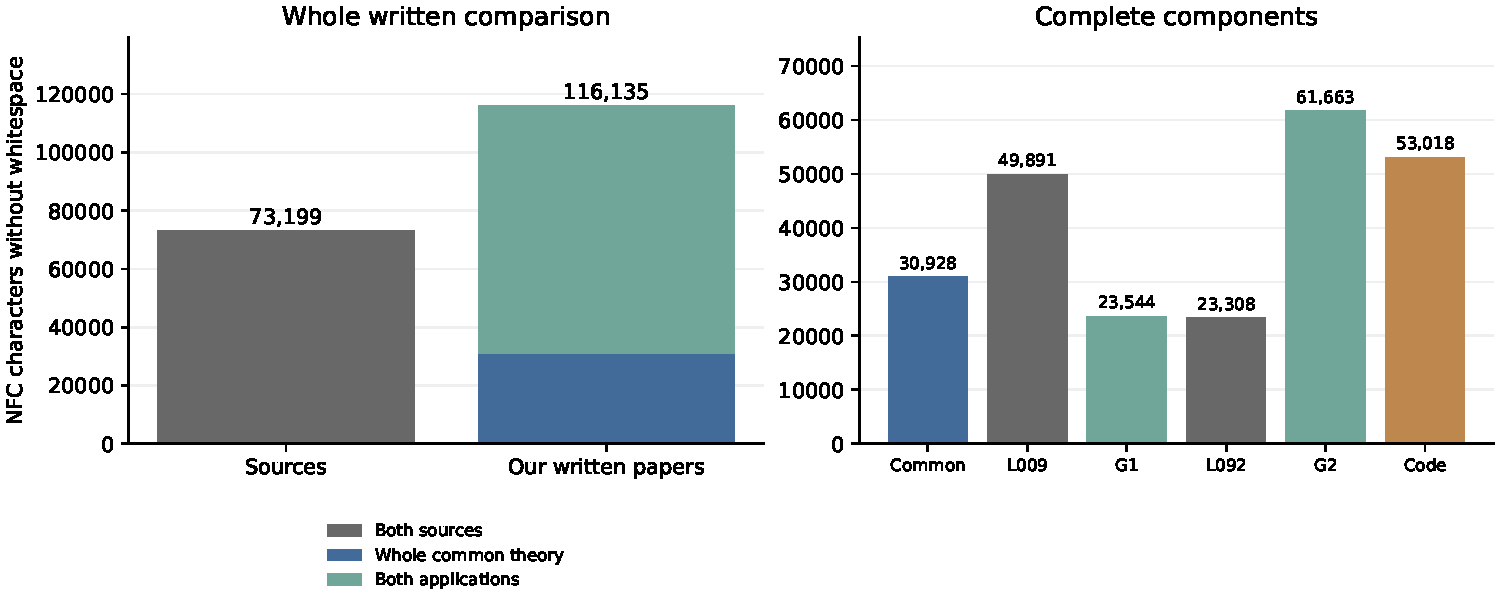
\includegraphics[width=\textwidth]{complete_costs.pdf}\end{center}
The left panel compares complete written totals. The right panel displays
all common, source, application and printed-program costs separately.
These lengths do not establish a recurring sawtooth pattern or minimum
mathematical proof complexity.

\paragraph{Sensitivity.}
For calibrated selected text with NFC normalization:
\begin{center}\begin{tabular}{lrrr}\toprule
Unit & Combined written & L009/G1 & L092/G2\\\midrule
Whitespace words & 0.728 & 2.513 & 0.499 \\
Alphanumeric units & 0.724 & 2.463 & 0.454 \\
Nonspace characters & 0.630 & 2.119 & 0.378 \\
Characters, collapsed spaces & 0.647 & 2.181 & 0.398 \\
UTF-8 bytes, collapsed spaces & 0.649 & 2.258 & 0.406 \\
\bottomrule\end{tabular}\end{center}
All five units are retained under NFC and NFKC for three extraction policies:
untrimmed raw, selected raw and calibrated selected. The thirty coordinates
supply 150 exact fractions: ninety combined and sixty conditional.
Removing only L009's identification cover gives the separately counted
article cost 49402. This changes the combined written factor to 0.626
and the L009/G1 factor to 2.098; L092/G2 is unchanged. The additional
120 exact fractions retain the printed and raw program alternatives too.
The primary comparison continues to include that cover.

\paragraph{Source qualifications and extraction.}
L009 retains the determinant correction and its circle-list, polarity and
ancillary-example limits. L092 retains the corrected deleted-line and
subline cases, path convention and Figure~2 qualifications; named-geometry
identifications and the claim without partial linearity remain excluded.
The full source texts are counted with these declared principal-result
contracts, not with an assertion that every historical statement is true.

The independent input audit checked all 101 physical pages, 180 PDF metric
cells and 220 separate raw-file cells. It aligned 75,909 source characters
with actual PDF text bytes and inspected the embedded glyph evidence.
The corrected cache identifies actual font dictionaries and effective
encodings: 701 occurrences had previously been mislabeled in the audit,
but none of the metric cells changed. The 509 visible-glyph calibrations
and all raw sensitivities remain explicit. The retained parsers are
pypdf 6.13.0 and fontTools 4.63.0; extraction does not price complete visual
information. Independent numerical review is required before publication.
\end{document}
